\documentclass[a4paper,10pt]{article}
\usepackage{graphicx}

%opening
\title{MIRACLE How-To}
\author{Andrea Mior, SIGNET Lab, University of Padova\\andrmior@dei.unipd.it}

\begin{document}

\maketitle

\begin{abstract}
All you have to know about main features of ns-MIRACLE in order to develop a simple project.
\end{abstract}

\section{MIRACLE}
MIRACLE is an extension for the ns2 simulator developed by the Department of Information Engineering at the University of Padova. The acronym stands for Multi InteRfAce Cross Layer Extension and describes one of its new capabilities intoduced by modularity. In fact, using MIRACLE you will be able to manage your nodes in a cross layer fashion and additionally multi technology support (whithin the same node) is provided.

\begin{figure}[ht]
\centering%
 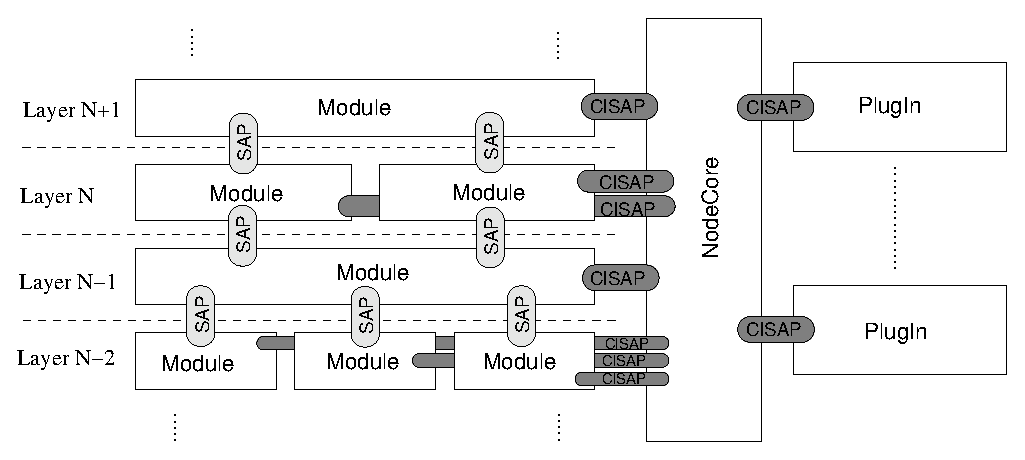
\includegraphics[width=10cm]{plugin.eps}
\end{figure}

The possibility of loading library dinamically has been introduced in standard ns2 simulator, starting from release 33. By now, we will suppose that you are using this simulator or a more recent one.

In MIRACLE every modification can constitute a stand alone library and can be loaded when necessary with the \verb=load= command. In this case modifications could be rapidly intercharged, loading the appropriate library. Furtermore a modification of a library requires only to recompile the code associated to that library and it usually requires some seconds. So you can save memory space (you need only a ns2 distribution) and precious time for debugging and simulations.

A motivation for creating the MIRACLE Extension is to fill the gap between ns2 and the simulation of multi technology enviroments and provide the possibility of performing cross layer messaging. This is one of the most advanced field of research and an opportune instrument for simulation is needed. The way MIRACLE reached this goal is a generic and technology independent approach.

MIRACLE node is based on generic entities connected by each other. The protocol stack is implemented through entities called \emph{Module}s. The novel idea consists in allowing presence of more than one \emph{Module} per layer. Every \emph{Module} is connected to another entity called \emph{Node Core}. It goes off the layer ordering scheme and has the task of coordinating message exchange between modules. It also stores the node actual position in the simulation field in order to allow position-dependent calculations such those related to propagation and interference models.

There are also another kind of entities connected to the \emph{Node Core}, called \emph{PlugIn}s. As \emph{Node Core}, they don't depend on layer classification. Due to their independence from the OSI stack, the \emph{PlugIn} may be exploited for node coordination functionalities (e.g., cognitive engines and multi interfaces manager) and cross layer intelligence.

Communication among different layers is provided by Service Access Points (SAP), accordingly to OSI structure.
As in ns2, connections between \emph{Module}s, \emph{NodeCore} and \emph{PlugIn}s are made by \emph{Connectors}, but the latter are completely reprojected to trace packets passing through them according to rules extablished by user.
%%Therefore we implemented a channel for the communication between module of adjacent layers such as defined in OSI structure, the Service Access Point (SAP). Thanks to the flexibility of the library, it is possible to define any number of modules in any layer and connect them to each other, by means of SAP. This help us in the design of architecture in which are involved multiple techologies for example. SAP are also used to implement the tracing of simulation activity, in fact, thanks to their strategic position, it is possible to trace with an ad hoc format all the packets exchanged between modules at each desidered level
%%



\section{Position Class}

This class manages informations about position of nodes whithin the simulation field. The two particular mobility models we'll see afterwards inherit from Position Class. This class exchanges with \verb=Node Core= informations which characterize the whole node and can be used at every layer of the protocol stack.
Node Core has the rule of provide and maintain node position informations. Every Module or PlugIn refers to Node Core for this kind of data. Position infos are managed by Position class.

In order to be able to operate on Position class objects, you have to declare class in the header file (*.h). So add:
\begin{verbatim}
#include "node-core.h"
\end{verbatim}
which tells to compiler where class is defined, and then explicitly recall the class name
\begin{verbatim}
 Class Position;
\end{verbatim}
at the beginning of the header file. Now your module knows how to manage this kind of data. Then insert the following lines in the *.cc file, when methods are defined:

\begin{verbatim}
Position* pos = getPosition();
printf("Position: %f %f\n", pos->getX(), pos->getY());
\end{verbatim}
There you call \verb=getPosition()= methods which immediately asks Node Core for position datas.
The rest of code allows you to print the current coordinates of your node. Methods \verb=getX()= \verb=getY()= return respectively the x and the y coordinate in the field.
We stress that what we presented above refers to the \verb=getPosition()= method. This belongs to PlugIn class, so only these kind of objects (e.g. Modules) can manage such data.

\section{Mobility models}
Node mobility in MIRACLE is ruled by two classes named BMPosition and GMPosition, derived from Position class. The former utilizes a Basic Movement (BM) model and the latter uses a Gauss-Markov (GM) model.

These models are those we provide with the MIRACLE release, but you can feel free to create your own!

The Basic Movement model moves nodes in uniform straightforward way. Nodes are moved by setting their destination by using the Tcl command \verb=setdest=, which accepts as inputs the coordinates of the destination and the speed (in meters per second) of the node. The true position of the node is updated only when needed, e.g. when the destination is changed or a calculation (as freespace attenuation or upon a \verb=getPosition()= call) is requested by an external module. In this model no control is added about borders of simulation field, so this means that a node, reached the setdest coordinates, will move in that direction and will not stop since a new destination is set.

The GMPosition Model is more complex than the previous one. In this case, nodes perform direction changes autonomously and a control of the behavior at borders is provided. Nodes adopting this mobility model requires mean direction (in radians) and a mean speed as inputs.

Speed and direction are calculated form mean values given as inputs multiplicating them by a random value, according to the following law (the law for direction is the same):
\begin{verbatim}
speed_ = (alpha_*speed_) + (((1.0-alpha_))*speedMean_) +
           + (sqrt(1.0-pow(alpha_,2.0))*Gaussian());
\end{verbatim}
As could be seen, the current (in this case) speed is calculated from previous value of speed and the mean speed, given as input. The incidence of the mean value is controlled by the \verb=alpha= parameter, which assumes values between 0 and 1. So the variations of speed are due to the ``old'' current speed and a random value provided by the \verb=Gaussian()= function.
It must be noticed that even if \verb=speedMean_= is 0, the current speed could be non-zero.
As in the previous model, position update is calculated when needed, but in this case every step from previous update is computed (because a gaussian walk is made of several gaussian steps). The time resolution of each step is provided by the \verb=updateTime_= variable.

There are four different behaviors for nodes reaching boundaries. These are \verb=REBOUNCE=, \verb=HARDWALL=, \verb=SPHERIC= and \verb=THOROIDAL=. In the first case the node rebounces on the border line, it means that if at least one of the coordinates exceeds the \verb=x= or \verb=y= field width it will be carried back in the field by a value equal to the difference between the exceeding coordinate and the field maximal coordinate. For example, if the simulation field is 100 meters wide and the new coordinate is 102 meters, then rebounce algo will carry back coordinate to 98 which is 100 - (102 - 100).

The \verb=HARDWALL= behavior expects that the node stops its movement at the border of the field, if trepassed. In case of \verb=SPHERIC= behavior the node will be put on the other side of the field, like an overflow. In the last case, \verb=THOROIDAL=, the node is put at the centre of the field.


\section{Packet Header Extension}

% [MM]: sure that this section is on packet payload?!? I guess that it treats mostly on packet header extensions instead of packet payload and Im scared that this may cause misleading in the reader. --> Changed section name
To transfer informations from one node to another, packets are sent over the channel. In the next section it will be described how to add custom data to the packets.

The ns2 class \verb=packet= provides methods to access the various fields of a packet. It has the \verb=setdata()= function that allows you to write in the data field of the packet, but the type of data you can write is AppData, and is very problematic to use expecially when using the \verb=copy()= method. We will not spend more time on it but we'll focus on a more useful way of data transportation.

Usually when you have to add some data to a packet you can add a field on existing headers or you can create your own header.

The first method is very simple and require small modification to the code, the second is al little bit more complicated.
Adding a new field on an existing header is possible adding the definition of the new field in the code where the header is defined. This is often positioned at the beginning of header files. Header of packet are defined as a \verb=typedef struct=. Your field can be inserted adding you data in the list preceded by the data type (e.g \verb=int numberOfPacketTransmitted_=). If you want, you can add a specific function allowing you to access that specific field. These functions are declared \verb=inline= and simply return a pointer to the field itself.

The creation of a personal header extends the procedure just seen. First thing to do is to create the packet header structure at the beginning of header (.h) file. Follow this example:

\begin{verbatim}
 typedef struct hdr_NC {
	 
	int len_;			/// \brief Lenght of the data field
	long gen_; 			/// \brief Generation of the packet
	double time_;			/// \brief Timestamp of the generation of the packet


	// Methods to access to the header fields
	inline	long& generation() { return (gen_);}
	inline	int& length() { return (len_);}
	inline	double& timestamp() { return (time_);}

	// Access to the NC header
	static int offset_;
	inline static int& offset() { return offset_; }
	inline static struct hdr_NC* access(const Packet* p) {
		return (struct hdr_NC*)p->access(offset_);
	}

} hdr_NC;
\end{verbatim}
As you can see, you have to add some lines at the end of the struct code. These lines are fundamental for the correct packet use. These metods provide a reference to the offset of header whithin the packet and a method to access the header structure, as we'll see in next paragraphs.

To make your header a valid header also for ns2 you have to decalre a class which inherits from \verb=PacketHeaderClass=. Usually this code is added in the initlib.cc file. With this definition, you make possible the creation of a header of the same size of the struct defined before. Using the access method defined in the struct you will able to access every single field of the header. The scheme is as follows, don't forget to define the offset and to include the header file where you defined the struct!
\begin{verbatim}
#include <tclcl.h>
#include "NCR.h"
int hdr_NC::offset_ = 0;

static class NCHeaderClass : public PacketHeaderClass {
public:
	NCHeaderClass() : PacketHeaderClass("PacketHeader/NC", sizeof(hdr_NC)) {
	 	bind_offset(&hdr_NC::offset_);
	}
} class_hdrNC;
\end{verbatim}
The file continues creating the header which will be added as overhead of packets
\begin{verbatim}
	...
extern "C" int Miraclencr_Init()
{
	NCHeaderClass* nc = new NCHeaderClass;  // <---
	nc->bind();				// <---

	InitTclCode.load();
	return 0;
}
\end{verbatim}
The last operation you have to do is to put the following string at the beginning of the file that set up default values of variables and/or provides description for Tcl procedures (for details on this kind of file, see Section \ref{makefile}). This string makes header ``active'' (i.e. tells to the simulator to reserve some memory space for it).
\begin{verbatim}
 PacketHeaderManager set tab_(PacketHeader/NC) 1
\end{verbatim}
This parameter is very important and often is a source of errors. Without setting \verb=tab_= you overwrite other header fields!

After the library compilation, you can see that (usually) in initTcl.cc file the new string is at the top of the file.

In this paragraph it will be explained how to manage the packet header in your methods. First thing to do is createing the packet at the sender side, allocating some memory space:
\begin{verbatim}
   Packet* p = Packet::alloc();
\end{verbatim}
This allocation is needed only if you are creating a new packet. In most of methods, you will refer to an existing pointer of a packet previously declared, such as those pointed by \verb=recv(Packet* p)= methods.

Then access the header and modify the field you are interested in:
\begin{verbatim}
  hdr_cmn* ch = hdr_cmn::access(p);
  ch->uid() = uidcnt_++;
  ch->ptype() = PT_MCBR;
  ch->size() = pktSize_;
\end{verbatim}
In this case we acessed the common header, which is a general scope header. We modified the sequence number, the packet type and packet size.

At the receiver side we manage incoming packet with the same procedure. We access a particular header for first and then we use one of the methods implemented to retreive the values of each field.
\begin{verbatim}
  hdr_ip* iph = hdr_ip::access(p);
  if (iph->saddr() != dstAddr_)
    {
      drop(p,1,CBR_DROP_REASON_WRONG_SADDR);
    }
\end{verbatim}
In this example we accessed IP header and then we checked the coherence of reception, evaluating if the packet is from the right sender. In this case the source addres is recovered by \verb=iph->saddr()=.

In one of the previous lines we changed the packet type, but we didn't expalined how to define a new one.
The first step is to define a new packet type, adding the string \verb=packet_t PT_MCBR;= at the beginning of (usually) the initlib.cc.
Then, in the same file you have to add the new packet type to the list of known packets in ns2. This is done by a simple procedure:
\begin{verbatim}
extern "C" int Miraclencr_Init()
{
	...
	PT_NC = p_info::addPacket("NC");

}
\end{verbatim}
This procedure automatically updates the list of packet types in ns2 code.

When you exploit the newly defined packet type, remember to insert at the beginning of the code you are going to use the call to the previously defined packet type writing \verb=extern packet_t PT_MCBR;=, so the program knows thath definition is provided in an \emph{external} file.

\section{CrLayMsg}

In this section we describe how to create and manage the Cross Layer Message, one of the most innovative advantages provided by MIRACLE framework. With these messages we are able to extablish a communication among modules of the node. They could be a request of some statistics from a layer (``give me the channel condition'') or a request to perform a particular action in another layer (``turn off radio!'' or ``Start handover!'').
% [MM]: I guess that is more interesting to use "channel condition" as example, cause usually packet SNR can be obtained the same thanks to its field in common packet header. --> OK
In our framework we are able to manage two kind of messages. These are \emph{Synchronous} and \emph{Asynchronous} messages. Both of them are created from the \verb=ClMessage= class but they differ in the way they are propagated within the node. Asynchronous messages are very similar to ordinary packet: a copy of the message is sent to each of the target module/plugIn. Syncronous messages are a bit different because the \emph-same- message is sent to all target modules. This means that the message is temporarily \emph{shared} with the sender and the receivers and therefore the instructions flow directly returns to the source when all the destinations have finished.
The two message types acquire the sinchronous or asynchronous property by the method used to propagate them among the node: you have at disposal the \verb-sendAsyncClMsg-(Up/Down) and the \verb-sendSyncClMsg-(Up/Down) PlugIn and Module classes methods. The former are more general methods, in fact they have to be used by PlugIn where there is no gerarchy information about the node, while the latter, in the brackets, are those of Module class and involve you choose a direction for your message

The message we are going to describe in more detail is the \emph{synchronous} message, often used to retreive informations among different layers. Synchronous means that interrogation and reply are in the same message and therefoer the answer is given sinchronously by the receiver(s).

To send a cross layer message we exploit a reference class named \verb=ClMessage=. Extending this class we create methods to manage our own messages.

In this example we consider an application layer and we'd like to collect some informations stored at layer 3.

We define the class name of this particular kind of message. We'll call it \verb=GetStats()= and it will manage the information retrieval. The sending starategy will be managed by another class.

We also define the name of this particular cross layer message as \verb=EXAMPLE_GETSTATS=. By convention, names of packet types and cross layer messages are always written in capital letters and spaces are replaced with underscores (\_).

We define a structure where informations will be stored. This structure is named \verb=Stats=. It constitutes the payload of the cross layer message.
% [MM] Here I can't get waht do you mean with "shape"...--> changed with payload

Going into detail, we expose the code of the \verb=ClMessage= constructor, which indicates how a \verb=ClMessage= must be formed (from clmessage.h).

\begin{verbatim}
 /**
	 * Standard ClMessage constructor.
	 *
	 * This constructor allows to set all the relevant
	 * parameters of ClMessage, and therefore can be used to
	 * create all types of messages (unicast, broadcast, layercast).
	 * 
	 * @param verbosity define the level of verbosity of the cross-
	 * layer message
	 * @param type define the type of the cross-layer message (this
	 * parameter is given by the simulator during the initialization
	 * phase, i.e., it is the value returned by the <i>addClMessage</i>
	 * method)
	 * @param dtype define the type of the destination (UNICAST or
	 * BROADCAST)
	 * @param value its intepretation is function of the <i>dtype</i>
	 * paramter:
	 * <ul>
	 * <li><i>dtype</i>=UNICAST:
	 * 	the id of the destination recipient</li>
	 * <li><i>dtype</i>=BROADCAST:
	 * 	the number of the layer to which the message has to be sent,
	 * 	or <i>CLBROADCASTADDR</i> if the message is directed
	 * to all the modules of the whole architecture</li> 
	 * </ul> 
	 *
	 **/


	ClMessage(int verbosity, ClMessage_t type, DestinationType dtype, int value);
\end{verbatim}
\vspace{0.6cm}

To form a message we need to properly set each field. Verbosity indicates how ``noisy'' the passage of the message will be across SAPs, then message will be identificated dinamically in each simulation by a \verb=type=. In our specific case we call it \verb=EXAMPLE_GETSTATS=. This is an important field cause it univocally identifies the new messages during each simulation run and therefore it allows their correct recognition at the receiving modules in order to make the appropriate procedures associated, in our case, the retrieval of particular statistics \verb=Stats=. Next field is the destination type, it could be \verb=BROADCAST= or \verb=UNICAST= and refers to the possibility of sending a message to a specific module or to every module of a layer. This aspect is perfectioned by the last parameter, \verb=value=, whose meaning depends by \verb=dtype=. If destination is \verb=BROADCAST=, this value indicates the layer to which message is addressed, if the destination type is \verb=UNICAST= the value denotes the identifier of the module which will receive the message. Be sure to not overwrite messages! In fact, in case you send a unique message in broadcast and there are many modules replying, they will write their answers on the same message!

In \verb=clmessage=\{.h,.cc\} code you can find also another constructor, which semplifies the operations of sending a message to the whole MIRACLE architecture. It it a method that automatically sets the \verb=dtype= parameter to \verb=BROADCAST= and also it sets the \verb=value= parameter to \verb=CLBROADCAST=, which allows the message to be received by all modules in all layers. In this constructor only message type and verbosity must be set.

Let's now create our own cross layer message class. We start defining the header file (*.h) for first. We'll call these files getstats\{.cc,.h\}. We define the struct that will house statistics and then it will characterize the packet.

\begin{verbatim}
typedef struct Stats
{
	// MAC level statistics
	double foo1_;
	double foo2_;
	// ...
};
\end{verbatim}

Suppose we want to retreive the values of two double variables from one of lower layers. We'll refer to them calling \verb=foo1_= and \verb=foo2_=.
Now we describe the \verb=GetStats= class, defining it as a class that inherits from \verb=ClMessage=, as seen before.

\begin{verbatim}
class GetStats : public ClMessage
{
	public:
		GetStats();
		GetStats(GetStats* m);
		GetStats(int verbosity, DestinationType dtype, int value);
		
		ClMessage* copy();	// copies the message
	
		Stats getStats();
		void setStats(Stats s);
	
	private:
		Stats stats_;
};

\end{verbatim}

We can see three constructors, a \verb=copy()= method and two other methods to manipulate data. At the end we declare a \verb=Stats= object which will house statistics. It is private so only this class (or friends) can modify its contents.

Now we'll describe each method, defining how it works.

\begin{verbatim}
// define message type
ClMessage_t EXAMPLE_GETSTATS = 0;

GetStats::GetStats() : ClMessage(STARTCAVERBOSITY, EXAMPLE_GETSTATS) {}
GetStats::GetStats(GetStats *m) : ClMessage(m)
{
}

GetStats::GetStats(int verbosity, DestinationType dtype, int value)
: ClMessage(verbosity, EXAMPLE_GETSTATS, dtype, value)
{
}

ClMessage *GetStats::copy()
{
	ClMessage *temp = new GetStats(this);
	((GetStats*)temp)->stats_ = this->stats_;
	return (temp);
}

Stats GetStats::getStats()
{
	return (stats_);
}
void GetStats::setStats(Stats s)
{
	stats_ = s;
}

\end{verbatim}
Constructors are responsible of the creation of the message, using the constructor mentioned before. Let's focus on next methods. The \verb=copy()= is fundamental, it is invoked every time your message crosses a SAP as an asynchronous message, so if you don't define this method, your message will not be able to correctly propagate within the node, since the value of the new added attributes are not copied. As previously discussed, when you call the \verb-sendAsyncClMsg- methods you send a copy of the same message to the adjacent SAPs.
Following methods are the core of the class and they define how to manipulate datas. In this case they are very simple, \verb=getStats= returns the structure with the data and \verb=setStats= assigns a particular set of value to the structure.

The last part of code regards the addition of the new cross layer message type to the list of known (and interpretable) cross layer messages. We previously declared \verb=EXAMPLE_GETSTATS= as a \verb=ClMessage_t= (in .cc file). To complete the process we have to add (usually) in the initlib.cc file the following code:

\begin{verbatim}
#include <tclcl.h>
#include <getstats.h>
extern EmbeddedTcl tclSupp;
extern ClMessage_t EXAMPLE_GETSTATS;
extern "C" int Miracle_Init()
{
	/*
	Put here all the commands which must be execute
	when the library is loaded (i.e. TCL script execution)
	Remember to ruturn 0 if all is OK, otherwise return 1
	*/
	EXAMPLE_GETSTATS = ClMessage::addClMessage();
	tclSupp.load();
	return 0;
}
\end{verbatim}
where we call the function \verb=addClMessage= to add the new message type.


Let's now show how it is possible to send synchronous messages over the node. On the sender side (the one who requests info) we have:
\begin{verbatim}
//message forming, note that is a GetStats message
		GetStats* m = new GetStats(DEFAULT_VERBOSITY, BROADCAST, 3);

//Sending message and synchronous reply (plugin.cc method)
		sendSyncClMsg(m);
//Now we have the reply and in m there is our structure stats_
//Reading the answer
		double FOO = m->getStats().foo1_;
\end{verbatim}

First thing to do is create an appropriate message, so we define \verb=m= as a \verb=GetStas= message directed to layer 3. Then we call the method \verb=sendSyncClMsg=, which is defined in plugin.cc. We point that each module inherits from Module class and Module class inherits from PlugIn class. This method is responsible of sending message from the module to the Node Core and then to the receiving module(s). Notice that, being message synchronous, the end of \verb=sendSyncClMsg= procedure means that we have a reply written on \verb=m=. At the end, we just recover the wanted info, and store, for example \verb=foo1_= in \verb=FOO= variable.

Now we explain what happens at the receiver side (the one who provides data requested), in this case a layer 3 module. If this destination module doesn't exist, the packet will be dropped.
\begin{verbatim}
int Layer3Module::recvSyncClMsg(ClMessage* m)
{
	if (m->type()==EXAMPLE_GETSTATS)
	{
		// Synchronous message -> answer directly in the message received
		// get the structure housed in the message
		Stats s = ((GetStats*)m)->getStats();
...
//fill required data fields (I'm writing on the message just arrived!)
		if (condition){
				s.foo1_ = statistic1;
				s.foo2_ = statistic2;
		}
//rewrite message content
		((GetStats*)m)->setStats(s);
		return 0;
	}
\end{verbatim}

As \verb=sendSyncClMsg=, method \verb=recvSyncClMsg= is a method derived from PlugIn class. It has the function of receiving synchronous ClMessages. To decide which actions to do and how to form response, we introduced an \verb=if= cycle where we evaluate message type. If it is an \verb=EXAMPLE_GETSTATS= message we know what variables the sender needs (in this case \verb=statistic1= and \verb=statistic2=) and in which format to send back datas (a \verb=Stats= structure). Every layer can potentially receive more than one cross layer message type from different layers, each one requiring particular informations and data format.

The next operation to do after the \verb=if= check is to get the structure contained in the incoming message, fill the correct fields and set the structure of the message with the newly created structure. Notice that we write the content of \verb=s= directly into \verb=m=, the incoming message. In this moment, the sender has statistics at its disposal as sender and receiver in this moment share the \verb=m= message.
The last note is about the two casts of \verb=m=. They are needed because \verb=recvSyncClMsg= accepts ClMessages to maintain generalization, in order to accept several kind of messages. So \verb=m= is interpreted as a ClMessage and a cast to \verb=GetStats= is needed.

\section{Timers}

% [MM]: The next sentence is a bit folkrositic...--> changed
If you are learning ns2, timers are often an obstacle. They concern with the ability of calling classes methods in consequence of an event schedule. The difficult raises when trying to find out in which order methods are called. If timers are involved, you can't expect to find nested calls of methods until the one you are interested in. In this section it is explained how to understand this behavior.

A TimeHandler, as name suggests, is an object created to manage time, and is defined in the common/timer-handler(.cc,.h) files of your ns2 distribution. This handler is in charge to schedule the execution of events during the simulation. The time the handler refers to is the simulation time, not depending on the time your machine uses to process the code.

A timer is like a state machine and is charachterized by three states. The first is \verb+TIMER_IDLE+ which means that timer can manage an event. The next state is \verb=TIMER_PENDING=, describing a status in which the timer is waiting to manage an event, and so it can't accept new events. This means that the timer has accepted to manage an event to be scheduled in the future and it is busy, waiting for this event. The last state is \verb=TIMER_HANDLING= in which the event is processed, calling the \verb+expire()+ function. After processing the event, timer returns in idle state.

In cbr/cbr-module(.cc,.h) of the MIRACLE distribution you can find a simple timer example, exploited to manage CBR packets transmission.

In the header file we define a new TimerHandler object. It is NOT possible to use TimerHandler class as is, because each timer has to handle its events in a particular fashion, which depends on the content of \verb=expire()= function.

\begin{verbatim}
/**
 * Timer used by CbrModule to schedule packet transmission
 */
class SendTimer : public TimerHandler
{
public:
  SendTimer(CbrModule *m) : TimerHandler() { module = m; }
	
protected:
  virtual void expire(Event *e);
  CbrModule* module;
};
\end{verbatim}

We defined the constructor, the \verb=expire()= function and a reference to the module the timer refers to.

On the other side, when defining CbrModule, we have to add \verb=SendTimer_= as a friend class, in order to make it able to properly manage events. In this case \verb=expire()= function has to call a CbrModule private method to activate packet sending processes.

\begin{verbatim}
  friend class SendTimer;
\end{verbatim}

It is also necessary to define (in CbrModule) the timer itself, to have a reference to the object to whom submit events.

\begin{verbatim}
  SendTimer sendTmr_;  /*timer which schedules packet transmissions*/
\end{verbatim}

In CbrModule.cc file, when you define the module constructor you have also to activate Timer constructor. This one has a reference to \textbf{this} to definitively associate \verb=SendTimer= to this \verb=CbrModule=. If you look at the definition of timer constructor, you'll see that it only associates a CbrModule to the object (the one which submits events) to be managed by the timer.

\begin{verbatim}
CbrModule::CbrModule() 
  : sendTmr_(this),
\end{verbatim}

At the top of the same file there is the definition of \verb=expire()= function. When timer switchs to the \verb=TIMER_HANDLING= state, it refers to this particular set of actions. When a CbrModule event expires, the function \verb=transmit()= is called. Note that this function is defined in \verb=CbrModule=, so Timer class has to be declaredas a  friend of Module one. The \verb=module= attribute refers to \verb=CbrModule=, as explained before (see the constructor).

\begin{verbatim}
void SendTimer::expire(Event *e)
{
  module->transmit();
}
\end{verbatim}

Now we are ready to schedule an event. \verb=TimerHandler= class offers two methods to do this. They work in a similar fashion: both of them schedule an event but, while one is made to be called occasionally (i.e., when the timer is not busy, \verb-TIMER_IDLE-), the second is created to work in an always pending status, in order to consecutively recall \verb=expire()= function. If timer is always in \verb=TIMER_PENDING= status, no other (sporadic) events can be managed by the timer. The former is called \verb=sched()= and the latter is called \verb=resched()=. The \verb-sched()- function works only if timer is \verb-TIMER_IDLE- while \verb-resched()- can potentially cancel a previously scheduled \verb-TIMER_PENDING- event and to schedule its new event. In this way the timer is maintaned always busy for those methods which don't call \verb-resched()- function. If your method instead, has the privileged \verb=resched()= call you can access and modify the events.

In \verb=CbrModule= we want to periodically transmit a packet. To achieve this result we use \verb=resched()= function.

\begin{verbatim}
void CbrModule::start()
{
  ...
  sendTmr_.resched(period_);
}
\end{verbatim}

At the end of \verb=transmit()= method we reschedule again an event in order to create a ``self-updating'' loop. In this case, at the end of expire function, we schedule the timer for next \verb=period_= instants, maintaining the loop.

\section{Tracer}

Tracers are files created to trace packets passing through SAPs. They are created for off-line statistical purposes and debug.

Creating a customized tracer for your needs is an easy procedure. You have to create a header file where define a constructor and a method, named \verb=format()=. This is the function called by each SAP when a packet get through it, so it is important that in every tracer you create a method with this name. The \verb=format()= function is always called passing a reference to the packet going through the SAP and a reference to the SAP itself as arguments.
Let's now explain how the Common Header Tracer works:
\begin{verbatim}
class CommonHeaderTracer : public Tracer
{
	public:
		/**
		 * The class constructor initialize the level to 1. This
		 * means that it will be the first Tracer which will 
		 * process the incoming packets
		 * 
		 * @see Tracer
		 **/
		CommonHeaderTracer();
		
		/**
		 * This method writes a string in the trace file:
		 *
		 * @param p pointer to the packet to be traced
		 * @param sap pointer to the SAP instance which ask for the trace
		 * 
		 **/

		// ad hoc tracer for common header
		void format(Packet *p, SAP *sap);

};
\end{verbatim}

The way you trace packets is then included in \verb=format()= method. Let's see how it is defined in .cc file. The first definition regards the tracer constructor. It inherits from \verb=Trace= class. You have also to add a parameter defining at which level of the stack you want to insert your tracer. In this case we see \verb=Tracer(1)=, so this tracer is positioned at first level. The next lines are dedicated to description of \verb=format()= function. It lies on \verb=writeTrace()= function. In this case we access the common header and then we write the info we need. When simulation ends, we'll find infos regarding all packet passed through SAPs stored in a tracefile.
\begin{verbatim}
CommonHeaderTracer::CommonHeaderTracer() : Tracer(1) {}

void CommonHeaderTracer::format(Packet *p, SAP *sap)
{
	//access the header
	hdr_cmn *ch = hdr_cmn::access(p);
	//write infos
	writeTrace(sap, "string %d", ch->value())
}
\end{verbatim}
where \verb=string= and \verb=ch->value()= have no meaning except for clarification.

To make the tracer active, you have to add your tracer to SAPs. You have to insert the following lines in (usually) initlib.cc file so tracers are loaded when you load your library. Notice that tracer can constitute a standing alone library, so they can be loaded on demand.

\begin{verbatim}
extern "C" int Trace_Init()
{
	...
	SAP::addTracer(new CommonHeaderTracer);
	SAP::addTracer(new IpHeaderTracer);
	...
	return 0;
}
\end{verbatim}

The last note is about the setting up of a trace file in Tcl. You have simply to define a trace file name variable and open a file, \verb=tf= in this case, with this name. Last command redirects the simulator trace output to your file.

\begin{verbatim}
set tracefname "/tmp/out.tr"
set tf [open $tracefname w]
$ns trace-all $tf
\end{verbatim}

When simulation ends, you have to terminate the trace update, writing last datas on file and then closing the tracefile.
\begin{verbatim}
$ns flush-trace
close $tf
\end{verbatim}

It is possible to create a Trace file for cross layer messages too. The procedure is the same, you always use the \verb=format()= function. The difference is in the \verb=initlib.cc= file: you have to add the tracer to a cross layer SAP and not to a simple SAP because cross layer messages travel through different paths than ordinary packets. All you have to do is replace \verb=SAP::addTracer(new ...)= with \verb=ClSAP::addTracer(new ...)=.

Sometimes you can encounter the BIN string on your trace files. It means that a packet had been dropped. It is often followed by an achronym that describes the reason of dropping.

Referring to \verb=cbr-module= files we'll explain how \verb=BIN= works. In header file you can find the definition of various dropping reason as:
\begin{verbatim}
#define CBR_DROP_REASON_UNKNOWN_TYPE "UKT"
\end{verbatim}

In the .cc file then we see how it is used. The key method is the \verb=drop()= function belonging to \verb=Module= class. It activates the packet tracing and deallocating procedure. For example, in \verb=cbr-module.cc= when we receive a packet we check if we can comprehend its content:
\begin{verbatim}
void CbrModule::recv(Packet* p)
{
  hdr_cmn* ch = hdr_cmn::access(p);

  if (ch->ptype() != PT_MCBR)
    {

      drop(p,1,CBR_DROP_REASON_UNKNOWN_TYPE);
      ...
      return;
    }
\end{verbatim}

Then the drop function moves packet to ns2 Bin function and traces the event, appending the drop reason. You can also define verbosity of drop tracing setting the second value of the \verb=drop()= function

An example of what you can see in a trace file is:
\begin{verbatim}
D 2.012392783 17 BIN LL SYN 23
\end{verbatim}

The capital D stands for ``Dropped'', then there is a timestamp, the node id and then you can read the rest as ``The packet number 23 was moved to Bin by Link Layer because MAC\_SYNC\_FAILED''.


\section{New Files, Default Values and Procedures}\label{makefile}

In this section we'll explain how to create a library from your own source code. After doing these steps you'll be able to load your modules, tracers, ecc. into simulation files.

What we have to do is create an automatic process to compile your source code, load default values and link them to the rest of simulator. All these parts will be encapsulated in the \emph{make} command.

Suppose that the name of new library will be \emph{foo}.

We will organize the new directory as follows:
\begin{description}
 \item[src subdirectory] it contains source files (*.cc, *.h) and files with default values and the files which loads default values (usually named initlib.cc) and the file containing default values itselves.
 \item[m4 subdirectory] containing \emph{nsallinone.m4} and \emph{nsmiracle.m4} files
 \item[autogen.sh file]
 \item[configure.ac file]
 \item[Makefile.am file]
\end{description}

% [MM]: Am I wrong or now there should be more stable link to this documents?!? --> mmmm...no
You can find \emph{nsallinone.m4} file here: \texttt{http://www.dei.unipd.it/$\sim$baldo/nsallinone.m4}. Put it in \emph{m4} subfolder.

Create a file named \emph{autogen.sh}, put it in the main directory and make it executable. The content of this file must be:
\begin{verbatim}
#!/bin/sh

aclocal -I m4 --force && libtoolize --force
      && automake --foreign --add-missing && autoconf
\end{verbatim}
remember to add the option \verb=-I m4=, which forces the file to search informations into \verb=*.m4= files.

Now create a file named \emph{configure.ac} and fill as follows:
\begin{verbatim}
AC_INIT(foo,1.0)
AM_INIT_AUTOMAKE
AC_PROG_CXX
AC_PROG_MAKE_SET

AC_DISABLE_STATIC
AC_LIBTOOL_WIN32_DLL
AC_PROG_LIBTOOL

AC_PATH_NS_ALLINONE

AC_DEFINE(CPP_NAMESPACE,std)

AC_CONFIG_FILES([
		Makefile
		src/Makefile
		m4/Makefile
		])
		
AC_OUTPUT
\end{verbatim}

Then create \emph{Makefile.am} file as here:
\begin{verbatim}
SUBDIRS = src m4
EXTRA_DIST = autogen.sh nsallinone.m4
ACLOCAL_AMFLAGS = -I m4
DISTCHECK_CONFIGURE_FLAGS = @NS_ALLINONE_DISTCHECK_CONFIGURE_FLAGS@


lib_LTLIBRARIES = libfoo.la

libfoo_la_SOURCES = foo.cc foo.h initlib.cc
libfoo_la_CPPFLAGS = @NS_CPPFLAGS@ 
libfoo_la_LDFLAGS =  @NS_LDFLAGS@
libfoo_la_LIBADD =   @NS_LIBADD@ 


nodist_libfoo_la_SOURCES = initTcl.cc
BUILT_SOURCES = initTcl.cc
CLEANFILES = initTcl.cc

TCL_FILES =  foo-init.tcl

initTcl.cc: Makefile $(TCL_FILES)
		cat $(TCL_FILES) | @TCL2CPP@ FooTclCode > initTcl.cc

EXTRA_DIST = $(TCL_FILES)
\end{verbatim}
This file is very important, it has a lot of informations. In the first part, we instruct compiler about files and directories which are necessary to complete linkage between your library and the rest of simulator. In the second part you define the name of the library (libfoo.la) and you provide the list of source code files which constitute the library itself (foo.cc foo.h and initlib.cc). initlib.cc file is the file the simulator refers to when library is loaded. It provides the list of opearations to be executed when library is loaded as packet header creation, Tracers setup and ClMessages setup.
FooTclCode is recalled in initlib.cc as we'll see afterwards.

There are also two more files: initTcl.cc and foo-init.tcl. The latter contains the default values of binded variables and eventually some Tcl procedures. The former is the transposition of the foo-init.tcl file into C strings and is automatically generated.

The last thing to define is the initlib.cc file structure. As we have just previously anticipated, this file has the structure presented in the following (remember that this is the minimum required to make library working, please refer to specific sections for code to insert to add a packet type or a tracer).

\begin{verbatim}
#include<tclcl.h>

extern EmbeddedTcl FooTclCode;

extern "C" int Foo_Init() {
	FooTclCode.load();
	return 0;
}
\end{verbatim}
Remember that the name of the C function has always the name of the library followed by \verb=_Init()=. Then there must be a call to \verb=load()= function and to \verb=return=.

We reassume the corrispondence that MUST be respected when creating files descripted above:

\vspace{1cm}
\begin{tabular}[c]{|l|c|c|}
\hline
what name & what file & where\\
\hline \hline
foo, lib. name & configure.ac & in \verb=AC_INIT=\\ \cline{2-3}
 & Makefile.am & lib\emph{libname} called 6 times\\ \cline{2-3}
 & initTcl.cc & \emph{libname}\_Init()\\
\hline
FooTclCode & Makefile.am and initlib.cc & name corrispondence in both files\\
\hline
initTcl.cc & Makefile.am & repeated 4 times\\
\hline
autogen.sh & Makefile.am & called in \verb=EXTRA_DIST=\\
\hline
\end{tabular}
\vspace{1cm}

Notice that the times a name is repeated (referring to the table above) is just indicative for a tipical set of configuration files. So you can find variations from previous table even in full working files.

And finally there is list of commands to create your loadable library and put all pieces together:
\begin{verbatim}
user@pcsignet08:~/foo$ ./autogen.sh
user@pcsignet08:~/foo$ ./configure --with-ns-allinone=/locale/ns/ns-allinone-2.33
                             --with-nsmiracle=<ns_folder_path>/
user@pcsignet08:~/foo$ make && make install
\end{verbatim}


Refer to \texttt{http://www.dei.unipd.it/$\sim$baldo/ns\_dl\_patch/Developer\_s\_manual.html} for more detailed informations.

As we mentioned afore, default values for variables and settings are stored in the file we called \emph{foo-init.tcl}. This contains default values for your variables. It is an important aspect, so take care. Starting a simulation with variables which have no value often means that they assume ``random'' values (i.e. the value of the variable(s) previously stored in that portion of memory). At simulation start you will be noticed of suc an event by a warning message. It has the form:
\begin{verbatim}
warning: no class variable Routing/MrclRoutingStatic::overheadLength_

        see tcl-object.tcl in tclcl for info about this warning.

\end{verbatim}

In the same file initialization of file headers are stored as we discussed regarding the \verb=tab_= variable. Being this a Tcl file it follows the rules of Tcl language so you'll set variable values by using the \textbf{set} command.

We now explain the content of one of these files, referring to the \verb=cbr-defaults.tcl= file, in \verb=cbr/= directory.

When you refer to a module in Tcl, you'll use the Tcl name for the calss. This name is defined in the *.cc file, in a part often described as ``TCL Hooks for the simulator''. In this case the file is \verb=cbr-module.cc= and the name is \verb=Module/CBR=. For example, let's set the value of \verb=packetSize_= variable when library is loaded:

\begin{verbatim}
Module/CBR set packetSize_      180
\end{verbatim}

Notice that this is a Tcl portion of code, so if you do the same on your simulation files, you'll obtain the same result: every module you'll create will use the value you defined in the line. It is important to emphasize that you are working on Tcl, so you can manage only those $C++$ variables you share with Tcl code. To do so you have to use the \verb=bind= command. Default values of other variables are only in $C++$, and their default values can be setted up in constructor as you see for \verb=txsn(1), hrsn(0), pkts_recv(0)= variables in \verb=cbr-module.cc= file.

% In this files you can also add some procedures === add something on \verb=instproc=

\section{Output Redirection}

This section describes a method to write some data on external files. This is not an aspect related directly to MIRACLE framework, but for a neophite it could be an useful tip.
This is an alternative use of \verb=printf= method. In this how-to we used this method to print datas or messages to standard output, but in this case we redirect output to a file.
The code is self-explaining, so we don't write anything but the comments.

\begin{verbatim}
// This is the file
	FILE *fd;
//this is the filename
	char filen[100];
//create a file named Nodo_<nodeId_>.out
	sprintf(filen,"Nodo_%d.out", nodeId_);
//open a file with name filen. New data is
//written at the end of existing file or a new one is created
	fd = fopen(filen,"a"); // "a" = append at the end of file
//writes on file fd
	fprintf(fd,"%f %f\n", now, statistica1_);
//closes files
	fclose(fd);
\end{verbatim}

For more documentation, refer to online tutorials on $C++$ such as those on www.cplusplus.com.

\section{Simulation Parameters}

As previous section, this one is dedicated to an aspect related to Tcl implementation and not to MIRACLE.
In these paragraph we'll explain how to insert some simulation parameters. You can do it by inserting them directly on the command line or pass them by a script.

The first difficulty we encounter is the format of the values given as input. They must be integers and sometimes this makes things a little more complicated. The solution is referring to an array of non integer values, so inputs will be the array indexes.

The structure of Tcl command is as follows:

\begin{verbatim}
set simNum_ [lindex $argv 5]
\end{verbatim}

With this line the variable \verb=simNum_= is set equal to the fifth parameter inserted from the command line (or executed by a script). Remember that numeration of parameters starts from 0, but the first parameter is always \verb=ns=, the command you use to start each simulation.

To avoid errors, we suggest to add always a control on the parameters inserted, as follows:

\begin{verbatim}
if {$argc != 6 } {
    puts "usage: $argv0 Nuser rate burstSize speed iter SimulationNumber"
    exit 1
}
\end{verbatim}

Sometimes it happens to insert less parameters than required caused, for example, by a space not welltyped (like this!).

The creation of an array is very simple. In the following lines we create an array composed by three elements which represent speed values in meters per second. Then, as seen before, we associate the third value inserted to a variable named \verb=s=. We'll use this one as the array index.

\begin{verbatim}
set speed(1) 0.55555555
set speed(2) 4.16666666
set speed(3) 0.0

set s [lindex $argv 3]

$position(3) speedMean $speed(s)
\end{verbatim}

In the last line we finally can set the mean speed of the node 3 by recalling the right value in our array. If you read the section about mobility and you have had a look at the code, you will easily recognize in this line the setting regarding a Gauss-Markov mobility model.

\section{FAQ}

CYGWIN

couldn't load libdei80211mr.so

HINT: \texttt{https://mail.dei.unipd.it/pipermail/nsmiracle-users/2008-March/000107.html}

\section{Notes}
\begin{itemize}

\item Remember that some are just conventions such as name of the file \emph{initlib.cc}. We emphasized these names putting in front of the file name the word \emph{(usually)}. Just respect coherence of the names as summarized in Table in Section \ref{makefile}

\item Remember to \verb=#include= the header files you need in your C++ files

\item Remember to load the appropriate libraries in Tcl files

\item Mailing List: \texttt{https://mail.dei.unipd.it/mailman/listinfo/nsmiracle-users}
\end{itemize}

\end{document}
